%%%%%%%%%%%%%%%%%%%%%%%%%%%%%%%%%%%%%%%%%%%%%%%%%%%%%%%%%%%%%%%%%%%%%%%%%%%%%%%%
% event_selection.tex: 
%%%%%%%%%%%%%%%%%%%%%%%%%%%%%%%%%%%%%%%%%%%%%%%%%%%%%%%%%%%%%%%%%%%%%%%%%%%%%%%%
\chapter{Event Selection}
\label{sec:event_selection_chapter}
%%%%%%%%%%%%%%%%%%%%%%%%%%%%%%%%%%%%%%%%%%%%%%%%%%%%%%%%%%%%%%%%%%%%%%%%%%%%%%%%

If a \WR boson and heavy neutrino \nul existed at a mass scale and coupling strength accessible 
at the LHC, evidence of them would manifest as an excess of events relative to expected backgrounds 
where two high-$p_{T}$ jets and two high-$p_{T}$, same flavor charged leptons were reconstructed.  
Charged leptons and jets were reconstructed and identified using the silicon tracker, the ECAL and 
HCAL, and the muon detectors.  In events where two same flavor charged leptons, and two jets were 
reconstructed, additional selections were applied to increase the sensitivity of this search to 
high-mass \WR and \nul signatures.

\section{Online Event Selection}
\label{sec:triggers}
Charged leptons that came from proton-proton interactions were identified by the trigger system.  Based 
on the multiplicity and energy of charged leptons, the trigger system selected events during 
collisions, and saved these events to permanent storage for further analysis.  The triggers presented 
here selected events in two steps.  In the first step, one or more Level-1 triggers were 
required to fire.  Then, in regions where Level-1 triggers fired, local reconstruction was run to 
build calorimeter and muon detector hits into granular, 3D energy clusters.  In the second step, 
a High Level trigger applied selection cuts to the 3D energy clusters.  If 
enough energy clusters (1 or 2, depending on the trigger) passed these selections, hits in the tracker 
layers were reconstructed into interaction vertices and charged particle tracks.  Track endpoints 
were then extrapolated along track trajectories to the calorimeters and muon detectors.  Extrapolated 
tracks that passed within $\Delta R < 0.1$ of an ECAL cluster were identified as electron (e) 
candidates, and extrapolated tracks that passed within the same distance of a muon detector cluster 
were identified as muon ($\mu$) candidates.  Final High Level trigger selections were applied to 
tracks in these e,$\mu$ candidates, and if the selections were passed the entire event was saved 
to permanent storage.  Specific selections used in different Level-1 and High Level triggers are 
discussed next.

Events used in the ee channel \WR search ($pp \rightarrow \WR \rightarrow eejj$) were first selected by Level-1 triggers 
that required: 

\begin{itemize}
	\item At least 40 GeV of energy was measured in one ECAL supercluster (SC), defined as a 5 $\times$ 5 crystal region.
	\item Or, at least 22 GeV of energy was measured in one SC, and at least 10 GeV of energy was measured in 
		another, non-overlapping SC.
\end{itemize}

Then, events were saved to permanent storage if the following double electron High Level trigger requirements 
were met: 

\begin{itemize}
	\item Two non-overlapping ECAL SCs were detected with energy $>$ 33 GeV.
	\item For each SC:
	\begin{itemize}
		\item The ratio of hadronic energy in the HCAL tower behind the SC to the SC energy was low, $\frac{E_{HCAL}}{E_{SC}} < 0.15$ in the barrel, $< 0.1$ in the endcap.
		\item For SCs in the barrel or endcap, 90\% of the SC energy was measured in an $(\eta, \phi)$ region that was two crystals wide in $\eta$.
		\item For SCs in the barrel, a reconstructed track with hits in at least two pixel tracker layers extrapolated to the $z_{SC}$ 
			SC center within 2.3 \cm, and the $(\eta_{SC}, \phi_{SC})$ SC center within the $(\eta, \phi)$ area of one ECAL crystal.
	\end{itemize}
\end{itemize}

The High Level trigger selections for electrons differ between the barrel and endcap regions because the ECAL 
crystal sizes and orientations relative to the $x$ and $y$ axes differ between the barrel and endcap, as 
explained in Chapter \ref{sec:experiment_chapter}.

A second set of ee channel events were used only to estimate backgrounds.  These events were first 
selected online using a Level-1 trigger that required $>$ 30 GeV of energy be measured in an ECAL SC 
with $|\eta| < 2.1$.  Following the Level-1 selection, events were saved to permanent storage if the 
following double electron High Level trigger requirements were met:

\begin{itemize}
	\item One SC was detected with energy $>$ 30 GeV.
	\item For the SC with energy $>$ 30 GeV:
	\begin{itemize}
		\item For SCs in the barrel or endcap, 90\% of the SC energy was measured in an $(\eta, \phi)$ region that was two crystals wide in $\eta$.
		\item The ratio of hadronic energy in the HCAL tower behind the SC to the SC energy was low, $\frac{E_{HCAL}}{E_{SC}} < 0.055$ in the barrel, $< 0.07$ in the endcap.
		\item In a cone of radius $\Delta R =$ 0.3 centered on the SC ($\thicksim$900 ECAL crystals, $\thicksim$35 HCAL towers in the cone):
		\begin{itemize}
			\item The fraction of the total ECAL energy in the cone not associated with the SC is low, $\frac{E_{ECAL}}{E_{SC}} < 0.225$ in the barrel, $< 0.121$ in the endcap.
			\item The total HCAL energy in the cone is small compared to the SC energy, $\frac{E_{HCAL}}{E_{SC}} < 0.155$ in the barrel, $< 0.16$ in the endcap.
		\end{itemize}
		\item For SCs in the barrel or endcap, a reconstructed track with hits in at least two pixel tracker layers extrapolates to the 
			$z_{SC}$ SC center within 1 \cm, and the $(\eta_{SC}, \phi_{SC})$ SC center within the $(\eta, \phi)$ area of $\frac{1}{2}$ ECAL crystal.
		\item For SCs in the barrel or endcap, the SC energy and the matching reconstructed track momentum cannot differ by more than 50\%
	\end{itemize}
	\item A second SC was detected with energy $>$ 4 GeV.
\end{itemize}


Events used in the muon channel \WR search ($pp \rightarrow \WR \rightarrow \mu\mu jj$) were first selected online using 
a Level-1 trigger that required $>$ 16 GeV of momentum be measured in a muon DT or CSC detector.  Following 
the Level-1 selection, events were saved to permanent storage if the following single muon High Level trigger 
requirements were met: 

\begin{itemize}
	\item The same requirements were applied to muon candidates in the barrel and endcap.
	\item A global curve representing a muon candidate was fit to a reconstructed track and at least one muon detector hit with $\chi^{2}/nDOF <$ 20.
	\item In the $(x,y)$ plane, the distance between the origin of the muon track and the primary vertex was $<$ 1 \mm.
	\item The reconstructed muon track had $p_{T} >$ 50 GeV.
\end{itemize}

A second set of $\mu\mu$ channel events were used only to estimate backgrounds.  These events were first 
selected online by a Level-1 trigger, which required $>$ 20 GeV of momentum be measured in a muon 
DT or CSC detector.  Following the Level-1 selection, events were saved to permanent storage if the 
following single muon High Level trigger requirements were met:

\begin{itemize}
	\item Unless noted otherwise, the same requirements were applied to muon candidates in the barrel and endcap.
	\item A global curve representing a muon candidate was fit to a reconstructed track and at least one muon detector hit with $\chi^{2}/nDOF <$ 20.
	\item In the $(x,y)$ plane, the distance between the origin of the muon track and the primary vertex was $<$ 1 \mm.
	\item The reconstructed muon track had $p_{T} >$ 22 GeV.
	\item In a cone of radius $\Delta R =$ 0.3 centered on the muon detector energy cluster ($\thicksim$900 ECAL crystals, $\thicksim$35 HCAL towers in the cone):
	\begin{itemize}
		\item The total ECAL energy in the cone is small compared to the muon cluster energy, $\frac{E_{ECAL}}{E_{\mu}} < 0.11$ in the barrel, $< 0.08$ in the endcap.
		\item The total HCAL energy in the cone is small compared to the muon cluster energy, $\frac{E_{HCAL}}{E_{\mu}} < 0.21$ in the barrel, $< 0.22$ in the endcap.
		\item The sum $p_{T,other}$ of all tracks in the cone excluding the muon track is small compared to the muon track $p_{T,\mu}$, 
			$\frac{p_{T,other}}{p_{T,\mu}} < 0.09$ in the barrel and endcap.
	\end{itemize}
\end{itemize}


As stated in Chapter \ref{wrBosonAndHeavyNu}, it is assumed that the $\WR$ decay cannot violate lepton 
flavor conservation.  As a result, the search presented here did not seek evidence of the LRS model in 
events with one electron, one muon and two jets in the final state.  However, events in the $e\mu$ channel 
($e\mu jj$ final state) were used to estimate backgrounds using a procedure described later.  The $e\mu$ 
channel events were first selected by a Level-1 trigger that required $>$ 16 GeV of momentum be 
measured in one muon DT or CSC detector.  Events that passed the Level-1 trigger were saved to permanent 
storage if the following electron $+$ muon High Level trigger requirements were met:

\begin{itemize}
	\item A global curve representing a muon candidate was fit to a reconstructed track and at least one muon detector hit with $\chi^{2}/nDOF <$ 20.
	\item In the $(x,y)$ plane, the distance between the origin of the reconstructed muon track and the primary vertex was $<$ 1 \mm.
	\item The reconstructed muon track had $p_{T} >$ 30 GeV.
	\item One ECAL SC was detected with energy $>$ 30 GeV.
	\item For the SC:
	\begin{itemize}
		\item The ratio of hadronic energy in the tower behind the SC to the SC energy must be low, $\frac{E_{HCAL}}{E_{SC}} < 0.15$ in the barrel, $< 0.1$ in the endcap.
		\item For SCs in the barrel or endcap, 90\% of the SC energy must be measured in an $(\eta, \phi)$ region that is two crystals wide in $\eta$.
		\item For SCs in the barrel, a reconstructed track with hits in at least two pixel tracker layers extrapolated to the 
			$z_{SC}$ SC center within 2.3 \cm, and the $(\eta_{SC}, \phi_{SC})$ SC center within the $(\eta, \phi)$ area of one ECAL crystal.
	\end{itemize}
\end{itemize}


\subsection{Data}
\label{sec:collisionData}

The LHC started colliding protons at $\sqrt{s} = 13\TeV$ center-of-mass energy in April 2015.  From 
April until mid August, proton bunches in each beam were separated by 50 \ns.  The data collected 
in this period, $\thicksim$0.2 fb$^{-1}$, was used to calibrate and align all CMS subdetector systems, but 
was not used in the search presented here for the following reason.  Before 2015 collisions began it 
was known that the amount of 50 \ns data collected would be small compared to the data collected with 
25 \ns bunch spacing.  As a result, the vast resources needed for physics analyses, like Monte Carlo simulations 
of SM processes used to estimate backgrounds, were only produced for data collected with 25 \ns bunch 
spacing.  The person-power needed to develop the same resources for 50 \ns data would have been 
detrimental to the quality of results produced with 25 \ns data.

The LHC stopped collisions in the second half of August and early September, evidenced by the plateau 
in Figure \ref{fig:lhc2015IntegLumi} \cite{lumi} during this time, to reconfigure the CERN accelerator system to 
deliver proton-proton (pp) collisions with 25 \ns between proton bunches.  The bunch spacing was decreased to 
increase the rate of pp collisions without increasing the number of interactions per pp collision event, 
which makes particle reconstruction and identification more difficult.  Collisions at $\sqrt{s} = 13\TeV$ 
resumed in September and continued until November 2015. During this period the LHC delivered approximately 
4.0 fb$^{-1}$ of data, but problems with the CMS magnet limited the amount of data recorded 
by CMS with the full 3.8 $\unit{T}$ magnetic field strength to 2.6 fb$^{-1}$.  The full 2.6 fb$^{-1}$ was used in this analysis, and was 
divided into two run periods - Run2015C and Run2015D.  All data from September until mid October 
was collected with similar beam conditions, like average instantaneous luminosity and the number of bunches 
per beam, and constituted run era Run2015C.  In mid October collisions stopped for $\thicksim$1.5 weeks for 
LHC maintenance, and to upgrade the LHC to deliver collisions with higher instantaneous luminosities, 
approaching $6 \times 10^{33} \frac{protons}{cm^{2}s}$.  Data collected after this upgrade and until the end 
of pp collisions in November constituted run era Run2015D.  As in Run2015C, all data in Run2015D was collected 
with similar beam conditions.  Comparing the two run eras in Table \ref{tab:collisionDatasets}, most of the 
data used in this analysis was collected in Run2015D.

\begin{figure}[h]
	\centering
	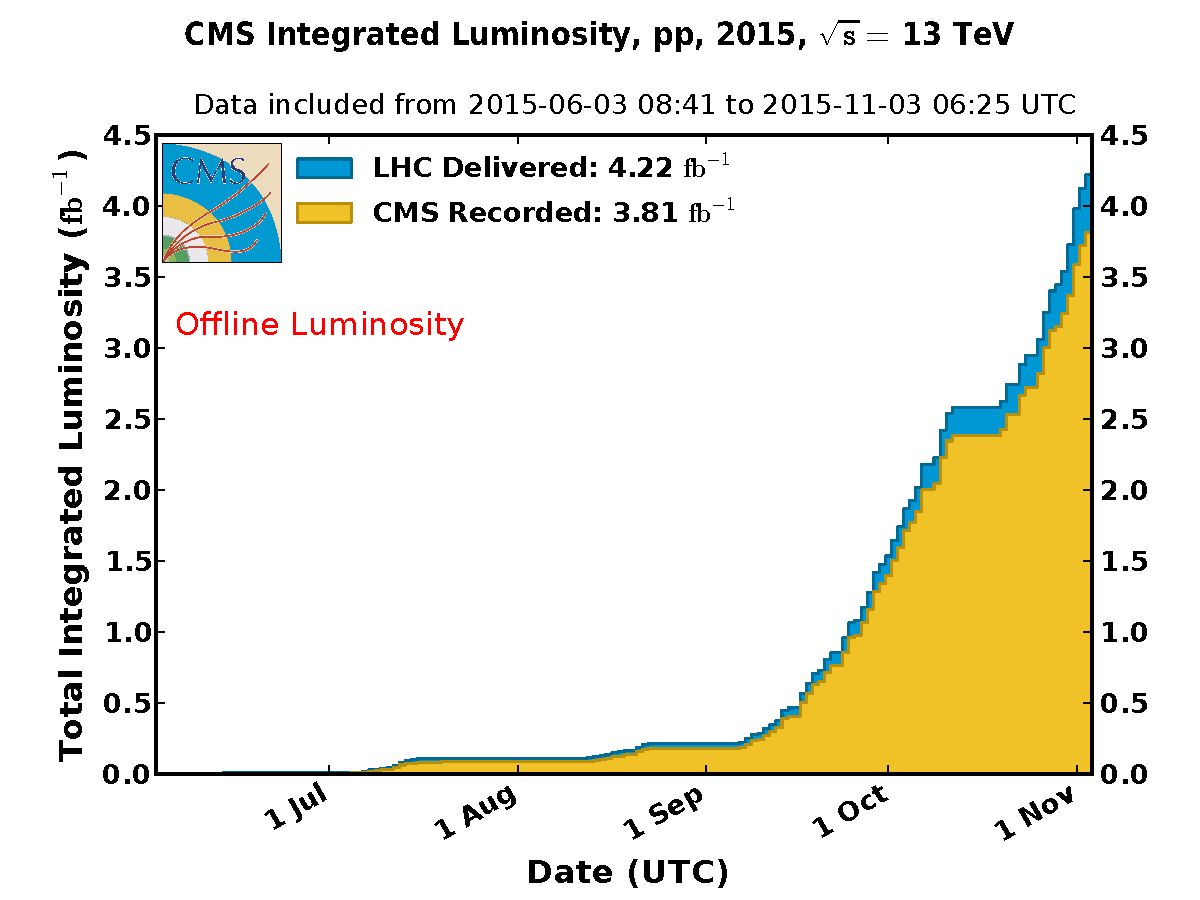
\includegraphics[width=1.0\textwidth]{figures/int_lumi_per_day_cumulative_pp_2015.pdf}
	\caption{Integrated luminosity delivered by the LHC and recorded by CMS in 2015.  Only data collected after 
	September 1st, corresponding to 25 \ns bunch spacing, was used in this search.}
	\label{fig:lhc2015IntegLumi}
\end{figure}

\begin{table}[h]
\caption{The amount of data collected in each run era.}
\label{tab:collisionDatasets}
\centering
\begin{tabular}{c|c}
Run Era & Int. Lumi (fb$^{-1}$) \\  \hline
	2015C &  0.02  \\
	2015D &  2.62  \\ \hline
\end{tabular}
\end{table}

After collision events were selected by High Level triggers, raw detector information was reconstructed into charged 
leptons, photons, and jets using procedures described later.  After the reconstruction process, the full 25 \ns 
2015 dataset collected by CMS was enormous ($\gtrsim 10^{4}$ terabytes), and contained much 
more information than what was needed by any individual physics analysis.  To expedite the transformation of 
collision data into a public physics result, reconstructed collision events from each run era were split into smaller 
datasets distinguished by the High Level triggers that selected the events.  As discussed earlier in 
Section \ref{sec:triggers}, collision events used in this analysis were selected if they had energy deposits consistent 
with at least one muon, at least two electrons, or at least one muon and one electron.  Events selected by the single 
muon triggers were assigned to the "SingleMuon" dataset, while those selected by the double electron and electron $+$ 
muon triggers were assigned to the "DoubleEG" (EG for electron gamma) and "MuonEG" datasets, respectively.  
The storage space consumed by these datasets largely came from object collections, representing quantities 
like individual hits in all tracker or calorimeter cells, that were not needed by the majority of physics 
analyses, including the one presented here.  Slimmed datasets were made by removing these object collections, and moving 
their important information into more general object collections, like the sole collection representing all 
reconstructed electrons.  Slimmed versions of the three datasets mentioned earlier were used in this 
analysis, and in each run era individual datasets were $\thicksim$5 terabytes or smaller.


%In addition to the trigger requirements discussed above, collision datasets are cleaned of events
%in which global reconstruction problems occurred within the detector.  These include events
%where no primary vertex is reconstructed, and when anomalous noise appears in the
%tracker, calorimeters, or muon detectors.  Furthermore, events identified as coming from
%interactions between a single proton beam and beam pipe gas or other foreign material are
%removed.


\section{Monte Carlo}
\label{sec:MC}

Monte Carlo (\MC) simulations were used in this search to model two types of processes.  The first 
type was Standard Model (SM) processes that resulted in the reconstruction of two charged leptons 
and two jets.  These included processes that produced two real charged leptons and two jets, like 
$pp \rightarrow Z+jets \rightarrow ll+jets$, and processes that produced multiple jets that 
were incorrectly reconstructed as charged leptons, like $pp \rightarrow W+jets \rightarrow l\nu+jets$.  
The second type was the \WR signal process $pp \rightarrow \WR \rightarrow l\nul \rightarrow lljj$ 
with different \mWR and \mnul masses.  
\MC simulations of both types of processes were produced by the CMS \MC production group 
in the following five step procedure.  In the first step, a \MC generator, like \PYTHIA or \MADGRAPH, simulated 
collision events between two protons in a vacuum, without any magnetic field or CMS detector 
components.  In simulations, the generator accounted for:

\begin{itemize}
	\item The energy carried by each proton into the collision (6.5 \TeV).
	\item How the incoming proton energy was distributed amongst constituent quarks and gluons according 
		to parton distribution functions (PDFs).
	\item The masses of the \WR, \nul and all particles in the SM.
	\item The coupling strengths between fermions and the bosons that mediated interactions.
\end{itemize}

Any unstable particles produced in the interaction, like a $Z$ or \WR boson, decayed according to 
their branching fractions to other particles, and any free quarks or gluons that were produced were 
run through a hadronization simulation that emulates jet production described in Chapter \ref{wrBosonAndHeavyNu}.  In the second 
simulation step, the effect of multiple pp interactions observed in real collisions is simulated by 
overlaying simulations of randomly chosen SM interactions onto the primary events simulated in the first 
step.  All pp interaction processes in the SM were assigned a probability proportional to their cross section 
times branching fraction, then several processes were chosen randomly, and the events they produced after 
the first simulation stage were overlaid on the primary events of interest.  Inelastic pp scattering and 
other gluon mediated interactions have cross sections times branching fractions to purely hadronic 
final states that are several orders of magnitude greater than processes which produce charged leptons 
or photons, so most of the randomly chosen events only created additional hadronic jets in each event.  After 
this overlaying procedure, the second simulation step used GEANT4 \cite{geant4} to simulate the propagation of all particles in 
the CMS magnetic field, their interactions with everything in the CMS detector, and the response of 
photodetectors and charge collection devices to all particles.  Using the simulated detector response, 
the third step simulated the Level-1 and High Level triggers, and every event saved a list of High 
Level triggers that it passed.  Following the trigger simulation, the fourth step reconstructed tracks, 
interaction vertices, and calorimeter and muon detector energy clusters, and built these into higher level 
reconstructed objects representing charged leptons, photons and jets.  The same reconstruction software 
was used in simulations and real collisions, and details of jet, electron and muon reconstruction 
algorithms pertinent to this thesis are discussed later.  All new information produced in each of the first 
four simulation steps was saved in every event, but much of this information was not needed in most 
analyses, including the one presented here.  To expedite the analysis of \MC events, the fifth and final 
simulation step applied the same slimming procedure used on collision datasets described earlier, and 
created a \MC dataset with the same structure as the slimmed collision datasets.  This five step procedure 
was used to simulate the \WR signal process at different \mWR and \mnul masses, and the SM processes 
summarized in Table \ref{tab:centrallyProducedMC}.


\begin{table}[bt]
\caption{Fully reconstructed \MC samples produced by the CMS \MC production group.  Cross sections
	are calculated at next-to-leading order (NLO) unless noted otherwise.  The \DY and t$\bar{t}$+jets events
were produced with a dilepton mass $M_{LL} > 50 \GeV$ selection applied to the two
leptons coming from the hard interaction.}
\label{tab:centrallyProducedMC}

\centering
\resizebox{\textwidth}{!}{
	\begin{tabular}{ |c|c|c|c| } 
	\hline
	Dataset         & Step 1 Generator & cross section (pb) & Size (fb$^{-1}$)   \\
		\hline
		Inclusive DY+jets, $DY \rightarrow ll$ & \MADGRAPH   & 5991    & 1.51 \\ \hline
		DY+jets HT 100-200, $DY \rightarrow ll$ & \MADGRAPH   & 181.3    & 15.0 \\ \hline
		DY+jets HT 200-400, $DY \rightarrow ll$ & \MADGRAPH   & 50.42    & 19.3 \\ \hline
		DY+jets HT 400-600, $DY \rightarrow ll$ & \MADGRAPH   & 6.984    & 153. \\ \hline
		DY+jets HT $>$ 600, $DY \rightarrow ll$ & \MADGRAPH   & 2.704    & 369. \\ \hline
		\ttbar+jets $\rightarrow ll$+jets & \MADGRAPH  & 85.67    & 286. \\ \hline
		single t $\rightarrow$ leptons+jets  & \POWHEG & 80.95 & 20.8 \\ \hline
		single $\bar{t}$ $\rightarrow$ leptons+jets & \POWHEG & 136.0 & 24.3 \\ \hline
		$\bar{t}$+W   & \POWHEG & 35.85 & 27.6 \\ \hline
		t+W   & \POWHEG & 35.85 & 27.8 \\ \hline
		WW  & \PYTHIA & 113.8   & 8.73   \\ \hline
		ZZ  & \PYTHIA & 10.15   & 98.2   \\ \hline
		WZ  & \PYTHIA & 23.4   & 41.8   \\ \hline
		W+jets $\rightarrow l\nu$+jets & \MADGRAPH & 50270   & 1.44 \\ \hline
		$\WR \rightarrow l\nul$  & \PYTHIA & 1$\times 10^{-5}$ - 4.3 & 5$\times 10^{6}$ - 11.6   \\ \hline
		\end{tabular}
}
\end{table}

In simulations of SM processes, different \MC generators were used in the first simulation step.  
The \DY (DY)+jets, W+jets, and t$\bar{t}$+jets simulations used the \MADGRAPH \cite{madgraph} generator, 
the single top and top+W simulations used the \POWHEG \cite{powheg} generator, and the diboson (WW, WZ, ZZ) 
simulations used the \PYTHIA \cite{pythia8,Sjostrand:2006za} generator.  In all of these 
simulations, \PYTHIA was used to hadronize free quarks and gluons into jets with the NNPDF23 PDF set 
\cite{nnpdf}.  Events used from these \MC datasets were required to pass at least one of the High 
Level triggers described earlier.

The \WR signal process was simulated using the \PYTHIA generator and NNPDF23 PDF set, and following 
the assumptions stated in Chapter \ref{wrBosonAndHeavyNu}.  \WR signals in the $\mu\mu jj$ and $eejj$ 
final states were simulated independently, with \mWR increasing from 0.8 to 6 \TeV in increments of 
0.2 \TeV, and $\mnul = \frac{1}{2}\mWR$.  Events from the $\WR \rightarrow \mu\mu jj$ samples were 
required to pass the single \mu, $p_{T} > 50$ \GeV High Level trigger described previously, while 
$\WR \rightarrow eejj$ events were required to pass the double electron $E_{T} > 33$ \GeV High Level 
trigger.

As stated previously, in the second step of \MC simulations, simulated events from randomly chosen SM 
processes were mixed into the main events being simulated.  For each event simulated for the main 
process (\WR or SM), the number of secondary events mixed in were pulled from a Poisson distribution 
with mean 12.  The secondary simulated events emulated multiple reconstructed interaction vertices, 
or pileup, in real data, but the PU distribution observed in data did not match that in simulated 
events.  To correct for the PU discrepancy between data and simulations, a PU dependent weight was 
applied to every simulated event before any further analysis of simulated events.

Independent of the CMS \MC production group, I produced additional $\WR \rightarrow lljj$ simulated 
datasets using \PYTHIA.  Only the first simulation step was run, and the \PYTHIA configuration was 
identical to what was used by the CMS \MC production group.  Datasets were produced with 
$0.8 \leq \mWR \leq 4.0$ \TeV increasing in \mWR increments of 0.1 \TeV, and $0.025 \leq \mnul < \mWR$ \TeV.  
Using a procedure described later, these datasets were used to extrapolate \WR cross section limits 
versus \mWR to \WR and \nul exclusion limits as functions of \mWR and \mnul.


\section{Muon Reconstruction and Selection}
\label{sec:muonRecoAndSelection}
Muon reconstruction began with the reconstruction of tracks in the muon chambers and silicon tracker.  
Muons passed through the tracker and ionized charge in silicon layers, which was measured to determine 
their vertices of origin and momenta.  Charge measurements made in multiple layers allowed a radius of 
curvature to be measured, which further constrained muon momenta and helped distinguish muons from other charged 
particles.  Muons that reached the muon detectors ionized charge from the gas along their trajectories, 
and this charge was measured and reconstructed into muon detector tracks.  Following track reconstruction 
in the silicon tracker and muon detectors, two algorithms \cite{cmsMuonRecoRunOne} were used to identify muons that traversed 
one or both detector systems.  One algorithm started with a seed track in the muon detectors, and 
extrapolated the track back to the silicon tracker.  Then, tracks in the silicon tracker identified as 
muon tracks were compared to the extrapolated muon detector track.  If a silicon tracker track had a 
trajectory that matched the extrapolated muon detector track, the algorithm built a muon from the 
combination of the two tracks.  This algorithm was developed to maximize reconstruction efficiency of 
high $p_{T}$, and was complemented by a second algorithm that started with a seed track identified as a 
muon in the silicon tracker.  The second algorithm extrapolated the seed track to the muon detectors in 
the magnet return yoke, and compared the seed track to the muon detector tracks.  If a muon detector track 
had a trajectory that matched the extrapolated seed track, the algorithm built a muon by combining the two 
tracks.  The second algorithm was developed to maximize reconstruction efficiency of low $p_{T}$ muons, which 
were not always able to traverse multiple layers of the iron return yoke to be detected in multiple 
muon chambers.  In both algorithms, if multiple matching tracks were found, the track assigned to the muon 
was the one whose trajectory was the closest match to the extrapolated track.

In the search presented here, the momenta of reconstructed muons were determined using the "Tune-P" algorithm 
\cite{cmsMuonRecoRunTwo}, which was developed to improve the momentum resolution with which high $p_{T}$ 
muons were measured.  For every muon, this algorithm simultaneously runs four algorithms that try to measure 
the momentum and fit a track to the entire reconstructed muon with the lowest $\chi^{2}/nDOF$.  All algorithms used all available 
information from the silicon tracker, and combined muon detector measurements and tracker measurements in 
different ways.  The first algorithm used all muon detector measurements, but gave greater weight to silicon 
tracker measurements in the track fit and momentum measurement.  The second algorithm used equally weighted 
tracker and muon detector measurements to fit a track, and used infrequent but distinct electromagnetic showers 
in all muon chambers to determine the muon momentum.  The third algorithm only used measurements made in the 
first layer of muon chambers closest to the magnet solenoid, where the muon has traversed the least amount of 
material before being detected, in combination with the tracker measurements to fit a curve to the global muon 
path, and determine the muon momentum.  The fourth algorithm dynamically truncated the length of the curve 
fitted to the global muon path when a large energy loss caused the muon to dramatically change direction, 
and as a result used as few as one layer of muon chambers to determine the trajectory and momentum of a muon.  
After all four algorithms were run, the "Tune-P" algorithm assigned the momentum to the muon from the algorithm 
that yielded a track fit with the lowest $\chi^{2}/nDOF$ and $\sigma(p_{T})/p_{T}$.  This procedure improved 
the muon momentum resolution for $p_{T} > 200$ \GeV, which in general degrades as muon $p_{T}$ increases as 
shown in Chapter \ref{sec:experiment_chapter}.

Following the momentum determination, muons were required to pass a $p_{T}$ selection, and 
identification selections designed to reject muons that were produced by decays or interactions away from the 
collision point, or jets incorrectly reconstructed as muons.  These requirements were applied identically to events 
in data and simulations.  To increase sensitivity to a \WR signal relative to the SM backgrounds, all muons were 
required to have $\pt > 53$ \GeV.  As shown in Table \ref{tab:lowerMuonPt}, the sensitivity of this search decreased using 
a looser $\mu$ $\pt$ selection.  After the $\pt$ cut, muons were required to pass the following selections:

\begin{itemize}
	\item The track fit obtained from "Tune-P" included at least one muon chamber hit.
	\item The origin of the track fit obtained from "Tune-P" was within 2 (5) \mm of the primary vertex in the $x,y$ plane ($z$ axis).
	\item Muon detector tracks were reconstructed in at least two muon chambers.
	\item The relative $\pt$ error on the muon momentum from "Tune-P" was below 30\%, $\sigma(p_{T})/p_{T} < 0.3$.
	\item The track obtained from the initial muon reconstruction had at least one hit in the silicon pixel detector, and had 
		hits in at least five layers in the entire tracker.
	\item In a $\Delta R = 0.3$ cone centered on the muon track in the silicon tracker, the $\Sigma \pt$ of all 
		tracks in the cone not matched with the muon must be low compared to the muon $\pt$, $\frac{\Sigma \pt}{\mu \pt} < 0.1$.
\end{itemize}

\begin{table}[h]
	\caption{Signal/$\sqrt{Background}$ (S/$\sqrt{B}$) for $\mu$ $\pt$
		cuts using simulated \DY, t$\bar{t}$ and $\WR \rightarrow \mu\mu jj$ events
	with $\mWR = 2.2 \TeV$ and $\mnuR = 1.1 \TeV$.  Lowering the $\mu$ $\pt$ cut would worsen S/$\sqrt{B}$.}
	\label{tab:lowerMuonPtCuts}
	\centering
	\begin{tabular}{c|c}
		$\mu$ $p_{T}$ cut (\GeV) & S/$\sqrt{B}$ \\  \hline
		40 &  11.9  \\
		53 &  12.6  \\ \hline
	\end{tabular}
\end{table}

There were known differences between simulations and data that effected the reconstruction and selection efficiencies 
of muons.  These differences were corrected by applying weights to muons in simulated events, and energy 
corrections to muons in data and simulated events.  In general the muon triggers were more efficient in simulations than in 
collisions, so the weight of every simulated event was scaled down by a factor dependent on the $\pt$ and $\eta$ of the 
triggering muon.  For the $\pt > 50$ \GeV trigger used in the $\WR \rightarrow \mu\mu jj$ channel search, the 
correction factors applied to the triggering muon in simulated events are shown in Table \ref{tab:muTrgCorrs}.  
Based on the peak position and width of the dilepton mass distribution in $Z \rightarrow \mu\mu$ 
events in data and simulations, it was known that the muon energy scale and resolution differed between simulations 
and data\footnote{the peak position differed due to different muon energy scale calibrations, and the width differed 
because the muon energy resolution differed between simulations and data}.  The $\pt$ of muons in data were corrected 
based on their $\eta$, $\phi$, charge and initial $\pt$ to bring the muon energy scale in data and 
simulations into agreement.  Using the same kinematic variables, the $\pt$ of muons in simulations were corrected 
to bring the muon energy resolution into agreement between data and simulations.  These corrections were applied 
before the $\pt > 53$ \GeV cut mentioned earlier.  Additional weights were applied to every simulated muon 
to eliminate the difference in muon identification selection efficiency between data and simulations.  For 
any reconstructed muon this weight was always between 1.0 and 0.985, and the uncertainty on the weight 
was below 0.001.

\begin{table}[htp]
  \caption{The correction factor applied to the triggering muon, as a function of its $\pt$ and $\eta$, in simulated events.}
  \label{tab:muTrgCorrs}
  \centering
  \begin{tabular}{ccccc}
	  \hline
	  $53 < \pt < 140$ & & & & \\
	  $|\eta|$         & $< 0.9$ & 0.9 to 1.2 & 1.2 to 2.1 & 2.1 to 2.4 \\
	  \MC correction  & $0.971$ & $0.964$ & $0.961$ & $0.951$  \\
	  \MC correction uncertainty & $0.00079$ & $0.0021$ & $0.0013$ & $0.0043$  \\
	  \hline
	  $140 < \pt$ & & & & \\
	  $|\eta|$         & $< 0.9$ & 0.9 to 1.2 & 1.2 to 2.1 & 2.1 to 2.4 \\
	  \MC correction  & $0.971$ & $0.999$ & $0.999$ & $1.04$  \\
	  \MC correction uncertainty & $0.0076$ & $0.025$ & $0.015$ & $0.051$  \\
	  \hline
  \end{tabular}
\end{table}


\section{Electron Reconstruction and Selection}
\label{sec:electronRecoAndSelection}
Electron reconstruction started with the reconstruction of ECAL energy clusters.  Electrons that impinged 
on the ECAL showered and lost substantially all of their energy in 5 $\times$ 5 crystal superclusters (SCs).  
The SC reconstruction algorithm was optimized to detect real electron energy deposits, typically two crystals 
wide or smaller in $\eta$, but large in $\phi$ due to electron bremsstrahlung in the magnetic field and energy 
lost to interactions with the tracker, with high efficiency.  Independent of SC reconstruction, electron 
tracks were reconstructed from silicon tracker measurements using a specialized electron track reconstruction 
algorithm.  On average a relativistic electron that traverses the entire silicon tracker will lose 33\% of 
its initial energy to bremsstrahlung in the tracker hardware.  The dedicated electron track reconstruction 
algorithm took this significant average energy loss into consideration when building tracks from tracker 
measurements.  Following track and SC reconstruction, tracks were extrapolated to the ECAL, and each electron 
was formed from one SC and one or three tracks, whose extrapolated positions matched the ECAL SC.  Three track 
combinations were allowed because a hard scatter between an electron and the tracker could produce an $e^{+}e^{-}$ 
pair in the tracker with sufficient energy to reach the ECAL.  The energy of each electron was taken from 
the ECAL, but its $\eta$ and $\phi$ were obtained from the reconstructed track.

Following electron reconstruction and energy determination, electrons were required to pass a $p_{T}$ selection, 
and identification selections.  These requirements were applied identically to events in data and simulations.  
To increase sensitivity to a \WR signal relative to the SM backgrounds, all electrons were required to have 
$\pt > 53$ \GeV.  After the $\pt$ cut, electrons were required to pass the following selections to reject electrons 
that were produced by decays or interactions away from the collision point, or jets incorrectly reconstructed 
as electrons:

\begin{itemize}
	\item The extrapolated track position and SC seed crystal position differed by less than 1 crystal width in $\eta$, and 
		about 3 crystal widths in $\phi$.
	\item For endcap electrons ($1.567 < |\eta| < 2.5$), at least 90\% of the ECAL SC energy was measured in a 2 crystal wide 
		region in $\eta$.
	\item For barrel electrons ($|\eta| < 1.44$), at least 94\% (83\%) of the SC energy was measured in a 2 (1) crystal wide 
		region in $\eta$.
	\item The ratio of hadronic energy in the HCAL tower behind the SC to the SC energy was low, $\frac{E_{HCAL}}{E_{SC}} < 0.05 + 1/E_{SC}$ in the barrel, $< 0.05 + 5/E_{SC}$ in the endcap.
	\item In a cone of radius $\Delta R =$ 0.3 centered on the electron:
	\begin{itemize}
		\item The $\Sigma \pt$ of all tracks excluding the electron track was low, $\Sigma \pt < 5$ \GeV.
		\item The calorimeter energy $E_{ECAL + HCAL}$ in the cone not associated with the electron was low, 
			$E_{ECAL + HCAL} < 2 + 0.03\alpha + 0.28\rho$, where $\rho =$ the neutral hadron energy per unit $\eta,\phi$ area, 
			and in the barrel $\alpha = E_{T}$ of the electron, and in the endcap $= E_{T} - 50$ of the electron.
	\end{itemize}
	\item The electron track had hits in every layer of the silicon pixel tracker and inner silicon strip tracker, or all 
		but one of those layers.
	\item The distance $\Delta_{xy}$ between the electron track origin and primary vertex in the $x$, $y$ plane was small, 
		$\Delta_{xy} < 0.2$ \mm in the barrel tracker, or $\Delta_{xy} < 0.5$ \mm in the endcap tracker.
\end{itemize}

There were known differences between simulations and data that effected the electron reconstruction and selection 
efficiencies.  These differences were corrected by applying weights to electrons in simulated events, and energy 
corrections to electrons in data and simulated events.  The double electron $\Et > 33$ \GeV trigger had the same 
efficiency in data and simulations for reconstructed electrons with $\Et > 53$ \GeV, so no trigger correction 
was applied.  Based on the peak position and width of the dilepton mass distribution in $Z \rightarrow ee$ 
events in data and simulations, it was known that the electron energy scale and resolution differed between simulations 
and data.  The $\Et$ of electrons in data were corrected based on their $\eta$, $\phi$, initial $\Et$ and ECAL shower 
shape to bring the electron energy scale in data and 
simulations into agreement.  Using the same kinematic variables, the $\Et$ of simulated electrons were corrected 
to bring the electron energy resolution into agreement between data and simulations.  These corrections were applied 
before the $\Et > 53$ \GeV cut mentioned earlier.  Additional weights were applied to every simulated electron 
to eliminate the difference in electron reconstruction and identification selection efficiency between data and 
simulations.  The weight applied to all simulated electrons was 0.982 to account for differences in reconstruction 
efficiency, and an additional weight of 0.989 was applied to simulated electrons to account for differences in 
identification selection efficiency.  A systematic uncertainty of 0.02 was assigned to each weight to account 
for weight variations versus electron $\Et$ and $\eta$.


\section{Jet Reconstruction and Selection}
\label{sec:jetRecoAndSelection}
Jets produced in proton-proton collisions contained long lived charged and neutral hadrons, photons from 
$\pi^{0} \rightarrow \gamma\gamma$ decays, and charged leptons from heavy quark decays.  Jets were reconstructed 
by first reconstructing electrons, muons, photons, and charged and neutral hadrons.  Photons were reconstructed using the same algorithm 
used to reconstruct electrons, excluding matching ECAL SCs to reconstructed tracks.  On average, a hadron that 
impinged on the ECAL had one significant inelastic scattering interaction with an ECAL crystal before entering 
the HCAL.  As a result, reconstructing charged and neutral hadrons started with the ECAL.  A modified version of 
the electron SC reconstruction algorithm, with looser requirements on the $\eta$ distribution of energy 
in the SC, was used to reconstruct hadronic energy clusters in the ECAL.  Then, energy deposited in individual 
HCAL towers was reconstructed into tower clusters (TC), and independently tracks not consistent with muons or 
electrons were reconstructed using silicon tracker measurements.  Every neutral hadron was built from a TC, and 
an ECAL SC if a geometric match was found.  Hadron tracks were extrapolated from the tracker to the HCAL, and 
each charged hadron was built from a TC and geometrically matching track, and an ECAL SC if a geometric match 
with the track was found.  After all particles were reconstructed, jets were reconstructed starting with 
charged particle tracks.  In each event, charged particles that traced back to the interaction 
vertex with the highest track $\Sigma \pt$ (the primary vertex) were used to tag different jets and their 
directions.  Then, all charged particles from the primary vertex, and all photons and neutral hadrons in the event 
were placed in a list of jet constituent candidates, which was subsequently analyzed using the anti-$k_{T}$ 
algorithm \cite{antikt}.  This algorithm took the $i^{th}$ particle from the list of jet constituents, and
calculated the distance parameter $d_{ij}$

\begin{equation}
	$d_{ij} = min(k_{Ti}^{-2},k_{Tj}^{-2})\frac{\Delta^{2}}{R^{2}}$
\end{equation}

using the $j^{th}$ particle in the same list, where $\Delta$ is the angular separation between the $i^{th}$ 
and $j^{th}$ particle, R is 0.4, and $k_{Ti}$ is the $p_{T}$ of the $i^{th}$ particle.  If the $i^{th}$ particle 
had $d_{ij} > k_{Ti}^{-2}$ for all j, then the $i^{th}$ particle was a jet constituent and was removed from the 
constituent list and placed in a new list $L_{1}$.  This procedure was repeated for all particles in the list of 
jet constituents, then repeated for all elements in the new list $L_{1}$.  The iteration over all particles in 
the newly created list continued N times, creating N lists, until the lists $L_{N}$ and $L_{N-1}$ had the same 
number of elements.  At the end, jets were produced from clusters of individually reconstructed particles.

Once the jets were clustered, their raw energies ($ = \Sigma E$ of constituents) were corrected in several steps.  
Neutral hadrons produced by pileup interactions can still be clustered into jets, so the first correction reduces 
the energy of every jet in a data or simulations based on the jet area and the total neutral hadron energy density 
in the event \cite{pileup1,pileup2}.  Subsequently, energy corrections based on jet $\eta$ and $p_{T}$ 
were applied.  These corrections, derived from \MC and applied to jets in data and simulated events, brought the 
reconstructed jet $p_{T}$ into closer agreement with the true (quark-gluon level) jet $p_{T}$ across the entire
range of reconstructed jet $p_{T}$ and $\eta$.  A second set of $p_{T}$ and $\eta$ dependent energy corrections, 
derived from \MC and applied to data events, brought the jet response in data into closer agreement with the jet
response in \MC.  More details on jet energy corrections, such as the types of \MC events used to derive the 
corrections, can be found elsewhere \cite{jetpaper}.

After jets in data and simulation were reconstructed and corrected, jet identification and energy requirements 
were applied.  The identification criteria required each jet to have:

\begin{itemize}
	\item $|\eta| \leq 2.4$
	\item less than 90\% of its energy came from neutral hadrons
	\item less than 90\% of its energy came from photons
	\item at least 2 constituents (from reconstructed charged or neutral particles)
	\item more than 0\% of its energy came from charged hadrons
	\item at least one constituent was a charged hadron
	\item less than 99\% of its energy came from electrons
\end{itemize}

The identification requirements were used to increase the fraction of selected jets which originate from real hadronic 
activity.  After identification selections, all jets were required to have $\pt > 40$ \GeV to increase the sensitivty 
to \WR bosons relative to expected SM backgrounds.  As shown in Table \ref{tab:lowerJetPtCuts}, a lower jet $\pt$ cut 
increased SM backgrounds without a corresponding increase in \WR signal.

\begin{table}[h]
	\caption{Signal/$\sqrt{Background}$ (S/$\sqrt{B}$) for subleading jet $p_{T}$ 
		cuts using simulated \DY, t$\bar{t}$ and $\WR \rightarrow \mu\mu jj$ events 
	with $\mWR = 2.2 \TeV$ and $\mnuR = 1.1 \TeV$.  Lowering the cut would worsen S/$\sqrt{B}$.}
	\label{tab:lowerJetPtCuts}
	\centering
	\begin{tabular}{c|c}
		jet $p_{T}$ cut (\GeV) & S/$\sqrt{B}$ \\  \hline
		30 &  12.1  \\ \hline
		40 &  12.6  \\ \hline
	\end{tabular}
\end{table}


\section{\WR Candidate Selection}
\label{sec:wrCandSelection}
%Following individual selections on electrons, muons and jets, \WR candidates are builhhhhhhhhhhhhhhhhhhhhhhhhhkt
Following the reconstruction of and selections applied to electrons, muons and jets, a \WR candidate in every 
event in the $\mu\mu$ (ee) channels was built from the two highest $\pt$ ($\Et$) muons (electrons), and the two 
highest $\pt$ jets.  In the $e\mu$ channel used for background estimation, the highest $\pt$ muon and highest $\Et$ 
electron were used to build an $e\mu jj$ candidate.  To increase sensitivity to a \WR boson signal, one lepton 
was required to have $\pt$ or $\Et > 60$ \GeV.  In addition, to significantly reduce the \DY+jets and diboson 
backgrounds, the combination of the two leptons was required to have mass $\Mll > 200$ \GeV.  After these lepton 
selections, the following selections were applied to the two leading jets in each event to ensure they did not 
overlap with the selected leptons:

\begin{itemize}
	\item $\Delta R(\ell_{1}, j_{1}) > 0.4$
	\item $\Delta R(\ell_{1}, j_{2}) > 0.4$
	\item $\Delta R(\ell_{2}, j_{1}) > 0.4$
	\item $\Delta R(\ell_{2}, j_{2}) > 0.4$
\end{itemize}

Finally, \WR candidates were required to have mass $\Mlljj > 600$ \GeV to increase the sensitivity to \WR boson 
signals relative to SM backgrounds.  The selections thresholds, and the lack of other kinematic cuts like missing 
$\Et$ were chosen to maximize the selection efficiency in \WR signal \MC, and allow the results of this search to 
be interpreted by a wide range of LRS theoretical models.  Shown in Figure \ref{fig:wrRecoSelectionEff}, the 
full trigger and offline selection efficiency in fully reconstructed \WR signal \MC exceeded 50\% (70\%) in the ee 
($\mu\mu$) channel.  The ee channel had lower efficiency due to the gap in electron detection for $1.44 < |\eta| < 1.57$, 
and tighter identification requirements on electrons than muons.

\begin{figure}[h]
	\centering
	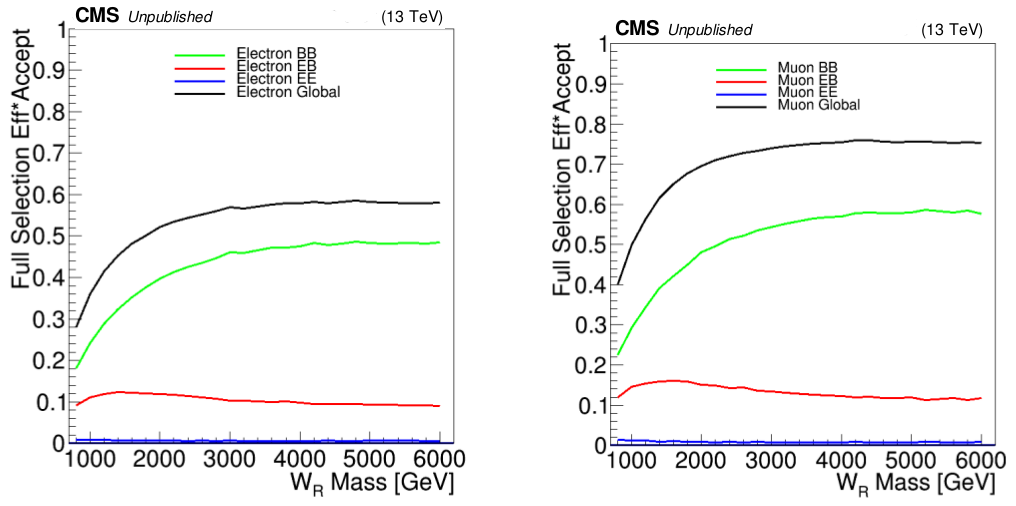
\includegraphics[width=1.0\textwidth]{figures/wrRecoSelectionEfficiency.png}
	\caption{The efficiency that $\WR \rightarrow \ell\nul \rightarrow \ell\ell jj$ events are selected using 
	the trigger and full offline selection in the ee ($\mu\mu$) channel on the left (right).}
	\label{fig:wrRecoSelectionEff}
\end{figure}

The $\Mlljj$ mass was chosen as the variable of merit because it clearly separates \WR signal from expected SM 
backgrounds.  Shown in Figure \ref{fig:mlljjVariableOfMerit}, a simulated \WR signal with masses $\mWR = 1.0, \mnul = 0.5$ 
\TeV was clearly differentiated from expected SM backgrounds as a sharp peak in the \Mlljj distribution.  This 
signal appeared in the low \WR efficiency region of this analysis, and higher mass signals were more clearly 
distinguished from backgrounds using the \Mlljj distribution.

\begin{figure}[h]
	\centering
	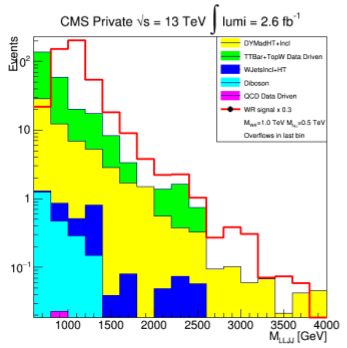
\includegraphics[width=0.5\textwidth]{figures/useOfLLJJMassAsFigureOfMerit.png}
	\caption{The $\Mlljj$ distribution from simulations of expected SM backgrounds and \WR signal in the ee channel.  
		The normalization of the \WR signal process is scaled down by 70\% only to better visualize the difference 
	between \WR signal and expected backgrounds.}
	\label{fig:mlljjVariableOfMerit}
\end{figure}



%%%%%%%%%%%%%%%%%%%%%%%%%%%%%%%%%%%%%%%%%%%%%%%%%%%%%%%%%%%%%%%%%%%%%%%%%%%%%%%%
